\section{Minimal Sensor Node}

\subsection{Introduction}
As a third device, I created a circuit that can collect environmental data with minimal energy consumption. These include brightness, temperature, humidity and depending on the sensor, a barometric pressure sensing function. A further consideration was to be lightweight and small so that it could be placed or attached anywhere to collect data.

\subsection{Minimal Sensor Node schematic diagram}
\begin{figure}[!htb]
    \centering
    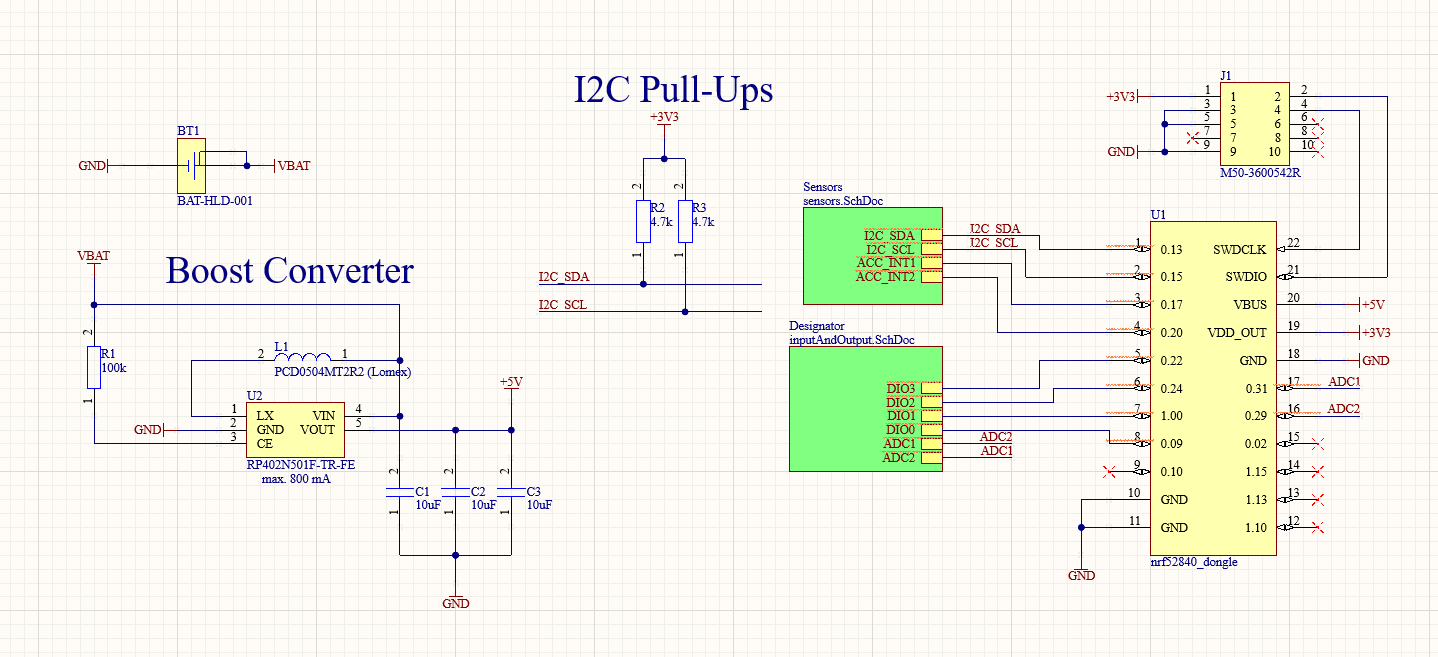
\includegraphics[width=\textwidth]{img/minimalsensornodeschematics.png}
    \caption{Minimal Sensor Node schematic}
    \label{fig:minimalsensornodeschematic}
\end{figure}

\begin{figure}[!htb]
    \centering
    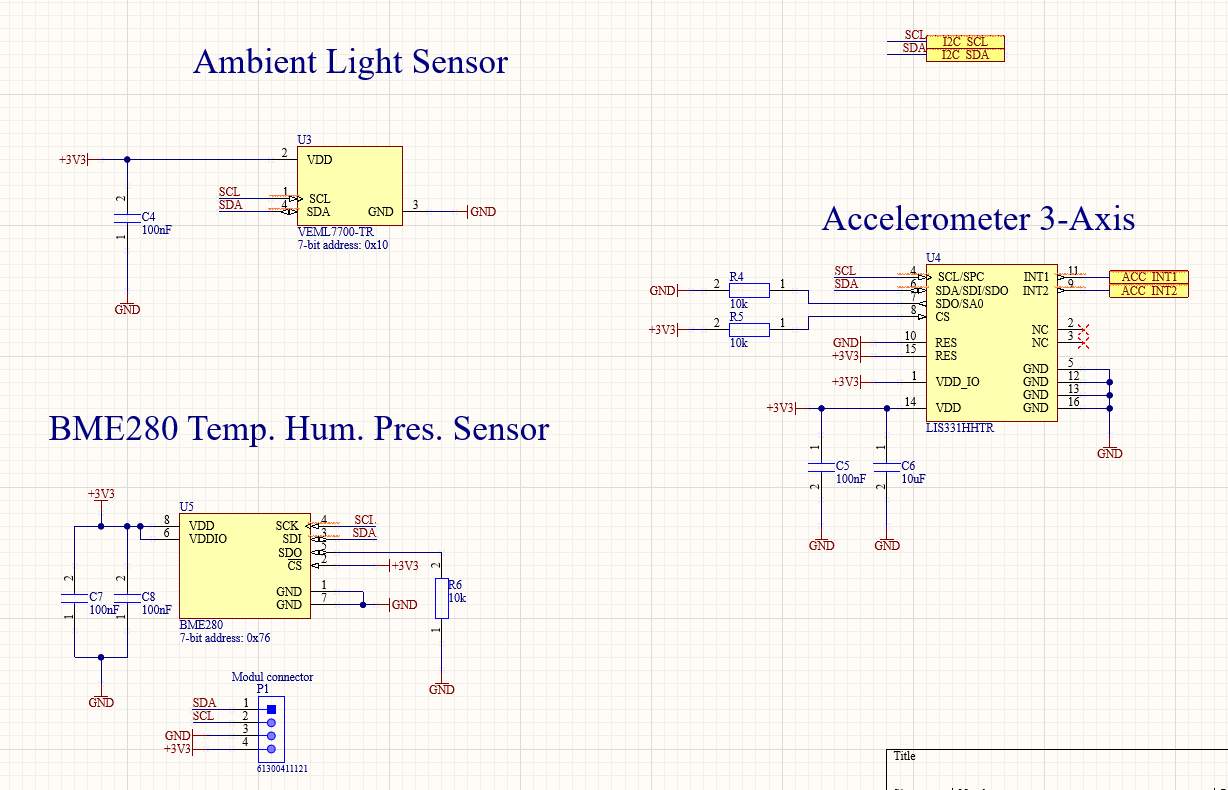
\includegraphics[width=\textwidth]{img/minimalsensornodeschematicssensors.png}
    \caption{Minimal Sensor Node schematic}
    \label{fig:minimalsensornodeschematicssensor}
\end{figure}
\noindent
Figure \ref{fig:minimalsensornodeschematic} shows the schematic of the Minimal Sensor Node. On the left side of the picture is a button coin cell battery holder, into which a CR2032 type 3V Lithium battery can be inserted. The dongle is designed for 5V power supply, so to avoid non-factory modifications to these modules, I saw fit to use a 5V boost converter using an IC with serial number RP402. This IC requires few elements (a couple of capacitors and an inductor) and has high efficiency. The right side of Figure \ref{fig:minimalsensornodeschematic} shows the nrf52840 dongle itself, connected to the outputs, inputs and sensors. Figure \ref{fig:minimalsensornodeschematicssensor} shows the sensor part of this node. I design 3 sensors for this device, one is a BME280 temperature, humidity and barometric pressure sensor, another is a VEML7700 light sensor and the third is a LIS331 3-axis accelerometer sensor.

\subsection{Minimal Sensor Node PCB design}
\begin{figure}[!htb]
    \centering
    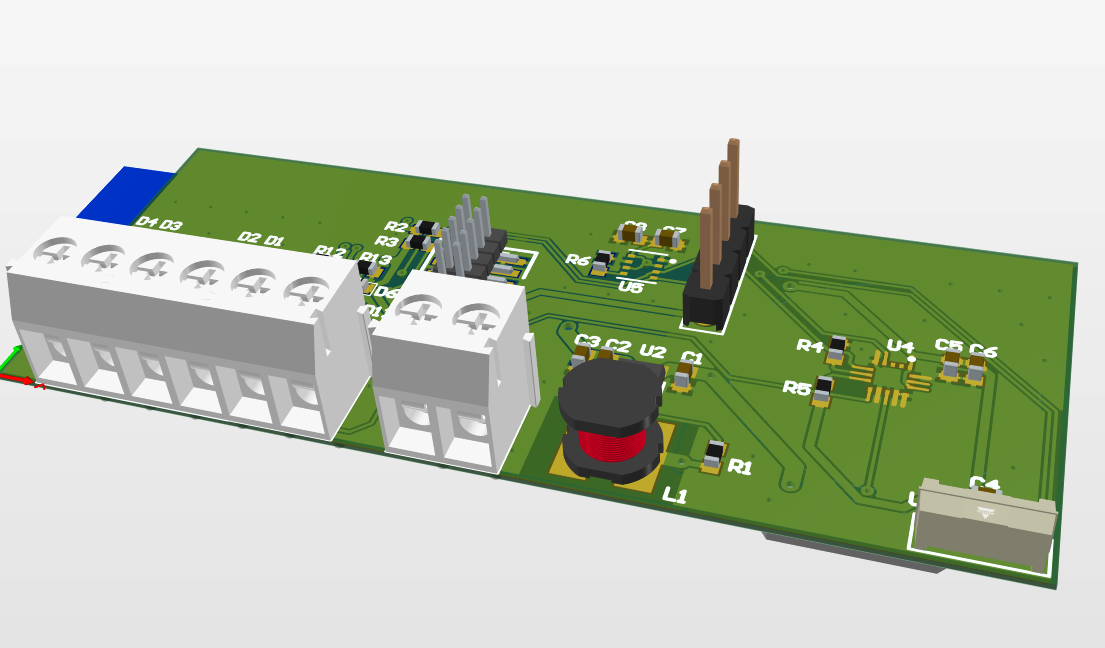
\includegraphics[width=\textwidth]{img/minimalsensornodepcb3dupper.png}
    \caption{Minimal Sensor Node - Upper side of PCB}
    \label{fig:powernodepcbup}
\end{figure}
\noindent
The PCB plan shows the top side where the sensors are located. The BME280 sensor is an LGA package, so I use a breakout board for it instead, which already has the pull-up resistors and filter capacitors for the unused pins of the chip. On the right side is the accelerometer and the VEML7700 light meter. In the Figure \ref{fig:powernodepcbup} the down side of this PCB is not shown, but there is the dongle module and the coin-cell battery holder.

\subsection{Webpage}
\begin{figure}[!htb]
    \centering
    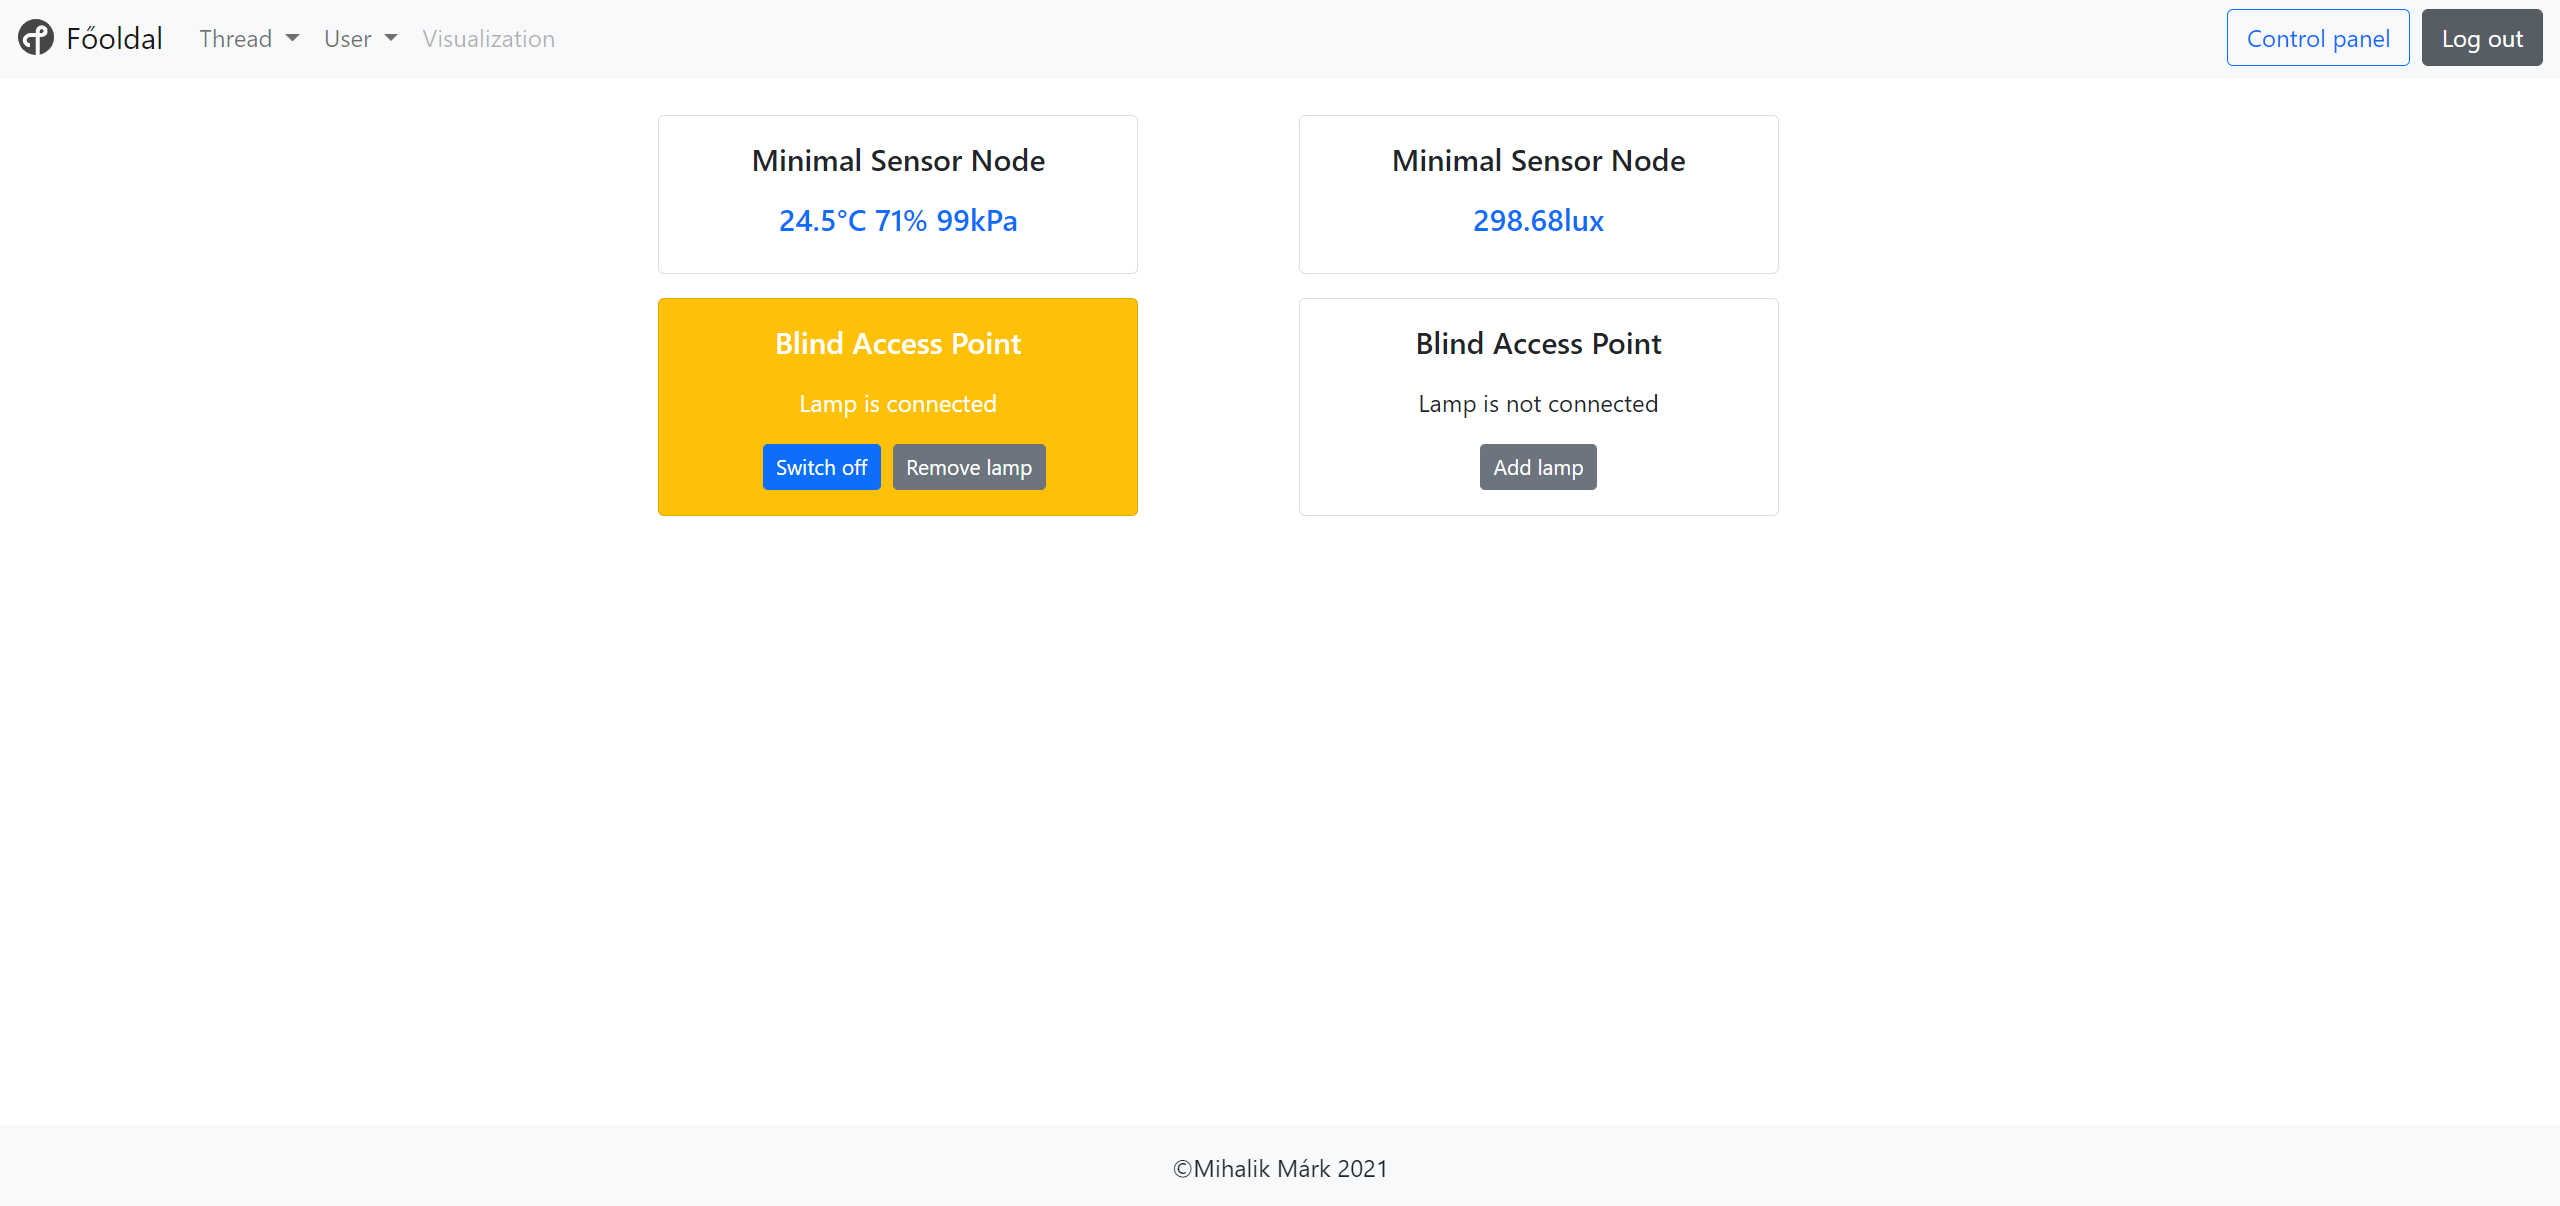
\includegraphics[width=\textwidth]{img/minimalsensornodeWebpage.png}
    \caption{Power Node PCB}
    \label{fig:powernodewebpage}
\end{figure}
\noindent
On the webpage there is the \textit{Minimal Sensor Node} on two different cards. In this moment this node can be used only with the BME280 or with the VEML7700. This is because Zephyr requires a specific driver, because its drivers split into parent and child. For example the parent is the I2C\_0 peripheral and the child consists of the sensors on the bus. I made the VEML7700 driver with the I2C\_0 peripheral, so I am not able to use the Zephyr BME280 driver, as I can not use the parent and child drivers together.

